\documentclass[pageno]{jpaper}
%\newcommand{\iscasubmissionnumber}{117}

\usepackage[normalem]{ulem}
\usepackage{booktabs}
\usepackage{mathtools}
\usepackage{ragged2e}
\usepackage{rotating}
\usepackage{array}
\usepackage{grffile}

\usepackage{epsfig}
\usepackage{float}
\usepackage{wrapfig}
\usepackage{setspace}
\usepackage{multirow}
\usepackage{graphicx}
\usepackage{fancyhdr}
%\usepackage{paralist}
%\usepackage{capt-of}

\usepackage{color}
\usepackage{xcolor,colortbl}
\usepackage{chngpage}
\usepackage{enumitem}
\usepackage{enumerate}
\usepackage{amsmath,relsize}
\usepackage[justification=centering]{caption}
\usepackage{tabu}
\usepackage{stmaryrd} % short right arrow

\usepackage{times}
\usepackage{fullpage}
\usepackage{tikz}
\usepackage{pgfplots}



\usepackage{listings}
\usepackage[makeroom]{cancel}


\usepackage{amssymb}% http://ctan.org/pkg/amssymb
\usepackage{pifont}% http://ctan.org/pkg/pifont
\usepackage[nomargin,inline,draft]{fixme}
\newcommand{\cm} {\clap{\small\ding{51}}\small\hphantom{--}}
\newcommand{\cmi}{\clap{\small\ding{51}-}\small\hphantom{--}}%
%\newcommand{\xm} {\clap{\ding{55}}\hphantom{--}}
\newcommand{\xm} {\clap{\small}\small\hphantom{--}}

\newcommand{\Forall}{\displaystyle\mathop\mathlarger{\mathlarger{\mathlarger{\forall}}} } 

%\newcommand{\cm} {{Y}}%
%\newcommand{\cmi}{{P}}%
%\newcommand{\xm} {{}}%


\usepackage{tikz,array}
\usetikzlibrary{calc}

%\newcommand*\circled[1]{\tikz[baseline=(char.base)]{
%            \node[shape=circle,draw,inner sep=2pt] (char) {#1};}}

%\newcommand*\ccircled[1]{\tikz[baseline=(char.base)]{
%            \node[shape=circle,draw,inner sep=2pt] (char) {#1};}}

\tikzstyle{every node}=[font=\footnotesize]

\newcommand{\hcancel}[5]{%
    \tikz[baseline=(tocancel.base)]{
        \node[inner sep=0pt,outer sep=0pt] (tocancel) {#1};
        \draw[black] ($(tocancel.south west)+(#2,#3)$) -- ($(tocancel.north east)+(#4,#5)$);
    }%
}%

\newcommand*\circled[1]{\tikz[baseline=(char.base)]{
            \node[shape=circle,draw,inner sep=0.5pt, minimum size=0.24cm] (char) {#1\vphantom{H}};}}

\newcommand*\ccircled[1]{\hcancel{\tikz[baseline=(char.base)]{
            \node[shape=circle,draw,inner sep=0.4pt, minimum size=0.24cm] (char) {#1\vphantom{H}};}}{-1pt}{1pt}{1pt}{-1pt} }


\begin{document}
\title{
\vspace{-0.15in}
\emph{Preliminary Draft -- Lot of pieces are still missing and needs to be added}
E-MOS: Efficient Energy Management Policies in Operating Systems
\vspace{-0.15in}
}



\author{Vinay Gangadhar \\ vinay@cs.wisc.edu \\ \and 
				Clint Lestourgeon \\ clint@cs.wisc.edu \\ \and  
				Jay Yang  \\ jkyang2@wisc.edu \\ \and
				Varun Dattatreya 	\\ channagirida@wisc.edu} 

\date{}
\maketitle

%\thispagestyle{empty}
\begin{abstract} \vspace{0.05in}

Power management in Linux is either handled by static, fixed policy power governors or Intel's P-state drivers. 
The former was designed to manage CPU idle states and scales frequency to do so while the latter was designed 
with the race-to-idle (or race-to-sleep) concept. Both of these solutions manage system power by changing the 
performance state of the CPU but they take a more holistic view of the system that could miss some of the nuances  
present in the active applications.

%Linux power governors operate on a generic energy management policy,
%based on the assumption that reducing frequency of CPU (using DVFS) or 
%putting the system to low-power state would reduce the system energy always,
%without having necessary information about the application. 
In this project, we explore the opportunities that application characterization presents for more efficient power management 
and provide an overview of the difficulties in Linux power management. 

We present E-MOS (Efficient Energy Management Policies in Operating Systems),
a power management model which uses applications characteristics (CPU/memory bound and cache sensitivity) to 
make frequency scaling decisions in order to achieve better energy efficiency while balancing the performance and energy requirements of a system. 
The decisions of this application aware policy 
can be applied through the ACPI (Advanced Configuration and Power Interface) userspace power governor. 
E-MOS is evaluated on variety of benchmarks and we see energy savings 
up to 2x for a 13\% performance loss.




\end{abstract}

\begin{comment}
Current Linux Operating Systems' power governors do not provide a fine-grained control and management 
over the energy utilized by the applications running on a computing system. 
Linux power governors by default use "Ondemand" CPU frequency governor for 
power management by considering the entire system load rather than individual application requirements. 
This system-wide and default kernel policy could have undesirable effects of OS power management 
and could lead to poor battery life and performance, 
at least for modern CPUs.
%Linux power governors operate on a generic energy management policy,
%based on the assumption that reducing frequency of CPU (using DVFS) or 
%putting the system to low-power state would reduce the system energy always,
%without having necessary information about the application. 
In this project, we provide an overview of the difficulties of Linux OS power management system and 
reason out the anomalies with different existing Linux power governors.

We present E-MOS (Efficient Energy Management Policies in Operating Systems),
a model which uses pre-characterized information of applications, to 
make decisions of frequency scaling to achieve 
better performance and energy efficiency. An application aware policy
can be applied using Linux User-space power governors, to
trade off performance and energy consumption. E-MOS is
evaluated on variety of benchmarks and we see energy savings 
up to X\% for a Y\% performance loss.

\end{comment}

\section{Introduction}\label{sec:intro}

\section{Motivation}\label{sec:motiv}

Modern multi-core computing systems (Laptops and hand-held devices) have major challenge of limiting the energy consumed by the system resources (CPU, Memory, Network) utilized when running applications. Most of the work on energy conservation in operating systems mainly rely on techniques which dynamically characterize power consumption and Quality of Service (QOS) of applications and provide a policy for users by using DVFS (Dynamic voltage frequency scaling)~\cite{dvfs} or lower-CPU power states~\cite{sleepscale, ecos}. 

Linux OS provide ACPI~\cite{acpi, freqgov} interfaces to extract information about batteries and other resources, but the power governors don't utilize this information efficiently to make proper energy management decisions. Current policies generally rely on user-specified static parameters to run at a specific lower CPU frequency or lower system power state without considering the applications’ requirements. Many multi-core processors try to improve the applications execution time by running at higher frequencies and thus consume more power (May consume less energy, if the execution time is small). Some applications have more memory accesses, in which case running at higher frequencies always is not beneficial. Many applications are long running jobs which consume lot of energy if run at higher frequency. All these above scenarios suggest that there is ‘NO’ one-size fit all solution for better system energy efficiency. Thus, Linux power governors need more application information, to determine whether to boost the performance or run at lower-power state by continuously monitoring the available battery resource. Our project aims to solve this problem of energy management decision by deriving some of the principles from Liang et. al~\cite{and-dvfs} implemented for Android systems.  



\section{Linux Power Governors}\label{sec:linux-powergov}

\if 0
\begin{figure}[h]
  \begin{center}
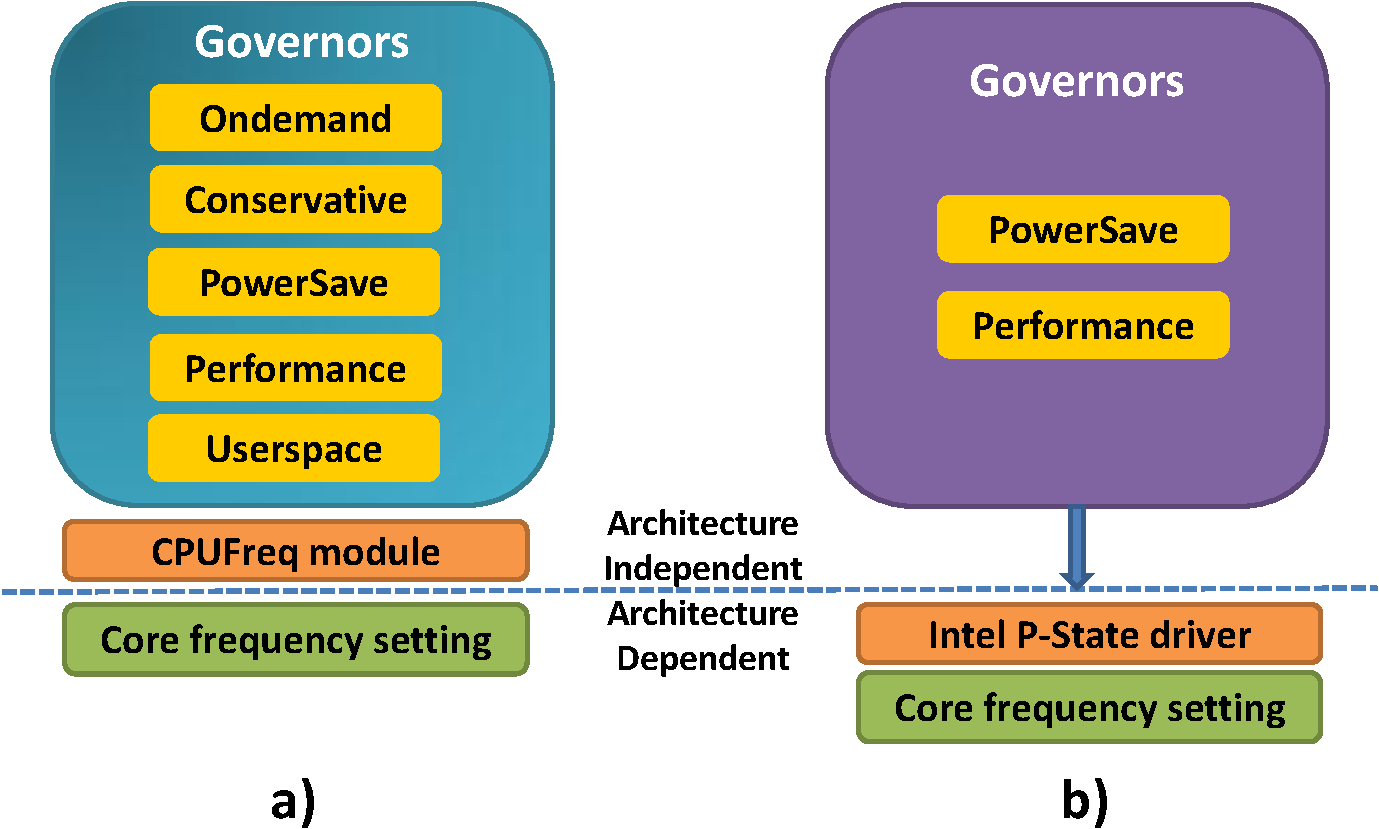
\includegraphics[width=\linewidth]{figs/gov-crop.pdf}
  \end{center}
  \vspace{-0.1in}
  \caption{Freq reduced by 30\%}
	\label{fig:gov}
\end{figure}
\fi

On today's Linux systems, depending on hardware availability and the version of the Linux kernel used in a distribution, power management 
is either handled by the ACPI governors or Intel's P-state drivers. The ACPI governors are platform independent solutions that base their decisions 
on system load and ACPI events and request CPU frequencies. On the other hand, Intel's P-state drivers were introduced in Linux 3.9 and support processors from Sandybridge onwards. 
The P-state drivers are more aware of the hardware capabilities of Intel's processors and request Performance states (P-states) rather than fixed frequencies.

\paragraph{ACPI governors}
These governors attempt to scale the CPU frequency in order to save power. CPU frequencies can be scaled automatically 
depending on the system load, in response to ACPI events, or manually by user space programs. The infrastructure available in Linux kernel to perform 
frequency scaling is called \emph{cpupower}.  

There are a number of ACPI governors available in Linux but the ondemand governor is the most widely used.
This governor sets the CPU frequency depending on the system load.  
In general, this governor tries to run the CPU load at high frequency. If the CPU load placed by the user abates, the Ondemand governor will slowly 
step back down through the kernel's frequency steppings until it settles at the lowest possible frequency, or the user executes another task to demand a ramp.
Ondemand scales its frequency in a work queue context. In other words, once the task that triggered the frequency ramp is finished, 
ondemand will attempt to move the frequency back to minimum. If the user executes another task that triggers ondemand's ramp, the frequency will bounce from minimum to maximum.

\paragraph{P-state drivers}
Intel's P-state drivers work on the race-to-idle concept. Since most modern CPUs consume very little power when idle, these drivers attempt to execute workloads as quickly 
as possible and return the CPU to an idle state. Race-to-idle policies benefit from the power savings of having the CPU in an idle state for most of the time. Apart from 
exploiting the idle CPU power savings, the P-state drivers are also aware of the available Performance states (or P-states), which represent a voltage-frequency operating point for the CPU. 
Currently, two P-state driver algorithms are selectable by the user: powersave and performance. As their names imply, the powersave driver emphasizes power savings at the cost of 
performance while the Performance driver works in a manner that is similar to the ACPI Ondemand governor.
 
\begin{comment}
\subsection{Performance}
This governor sets the CPU statically to a maximum frequency. This governor comes in handy in today’s phones, which implement a faster race to idle. Race-to-idle is the process by which a phone completes a given task, such as syncing email, and returns the CPU to the extremely efficient low-power state. This governor however, relies on a kernel that properly implements low power CPU C states.

\subsection{Powersave}
This governor is the opposite of Performance governor and sets the CPU statically to the lowest frequency set by the user.

\subsection{Userspace}
This governor allows the user or any user space program running with UID “root” to set the CPU to a specific frequency. This governor is more common amongst server and desktop PCs and is seldom used in mobile devices.

\subsection{On Demand}
This governor sets the CPU frequency depending on the current usage. To do this the CPU must have the capability to switch between frequencies very quickly. In general, this governor tries to run the CPU load at high frequency. If the CPU load placed by the user abates, the Ondemand governor will slowly step back down through the kernel's frequency steppings until it settles at the lowest possible frequency, or the user executes another task to demand a ramp.
Ondemand scales its frequency in a work queue context. In other words, once the task that triggered the frequency ramp is finished, ondemand will attempt to move the frequency back to minimum. If the user executes another task that triggers ondemand's ramp, the frequency will bounce from minimum to maximum.
This governor provides tunable parameters like sampling rate, the rate at which governor takes a look at CPU usage and makes a decision about frequency and sampling down factor, the rate at which the governor makes a decision on when to decrease the frequency while running at top speed

\subsection{Conservative}
This governor much like the ondemand governor, sets the CPU depending on the current usage.  It differs in behavior in that it gracefully increases and decreases the CPU speed rather than jumping to maximum speed the moment there is any load on the CPU. This behavior is more suitable in a battery powered environment.
This governor provides tunable parameters like frequency steps, which describes what percentage steps the CPU freq should be increased and decreased smoothly by.

\subsection{Min- Max}
This governor as the name suggests only makes use of minimum and maximum frequencies depending upon the CPU load and does not use any intermediate frequencies.

\subsection{Interactive}
Much like the ondemand governor, the Interactive governor dynamically scales CPU frequency in response to the workload placed on the CPU by the user. However, this governor is significantly more responsive than ondemand, because it's faster at scaling to maximum frequency.
Unlike Ondemand governor, which scales clock speed in the context of a work queue, Interactive governor scales the clock speed over the course of a timer set arbitrarily by the kernel. In other words, if an application demands a ramp to maximum frequency by placing 100\% load on the CPU, an user can execute another task before the governor starts reducing CPU frequency. The timer also renders this governor better suitable to utilize intermediate frequencies.
\end{comment}

\section{Imperfect Scaling Study}\label{sec:case-study}

This section focuses on a case study, which explores the frequency scaling 
capability of the system with two types of access patterns in applications.
An assumption often made, with respect to the power utilization 
is that on a given CPU, changing the frequency will change the CPU performance by the corresponding amount (generally called as scaling).
However, this is only true when considering the CPU execution. 
But, there are other architectural parameters whose performance do not scale along with CPU frequency.
One particular example would be memory. CPU caches hide much of this latency, but cache misses can be particularly damaging for the system energy efficiency,
as the time frame is too short for the operating system to handle the cache misses intelligently, or even be aware of them.
%except retrospectively, 
Yet, OSes take long enough time to make a decision that they measurably decrease the performance and/or efficiency.
 
To demonstrate this effect, we wrote a simple micro-benchmark, where a process takes large array (32MB), 
copies a random entry to another random entry in memory. 
We then operate the CPU at variety of frequencies using \texttt{CPUPOWER}~\cite{cpupower} utility and measured the execution time.  
This workload was then compared to another process that did the exact work of copying data from one point to another, but did so sequentially, avoiding most of the cache misses. 
As expected for both processes the time to execute decreases as CPU frequency increases.
We can then plot the \emph{efficiency}, computed  here as the time to execute the process
represented as the number of clock cycles per operation. For ease of comparison these were then normalized.
Figure~\ref{fig:case} shows the comparison of the random access workload with the sequential workload with increasing CPU frequency, normalized
to the base 1200Mhz frequency. 

\begin{figure}
  \begin{center}
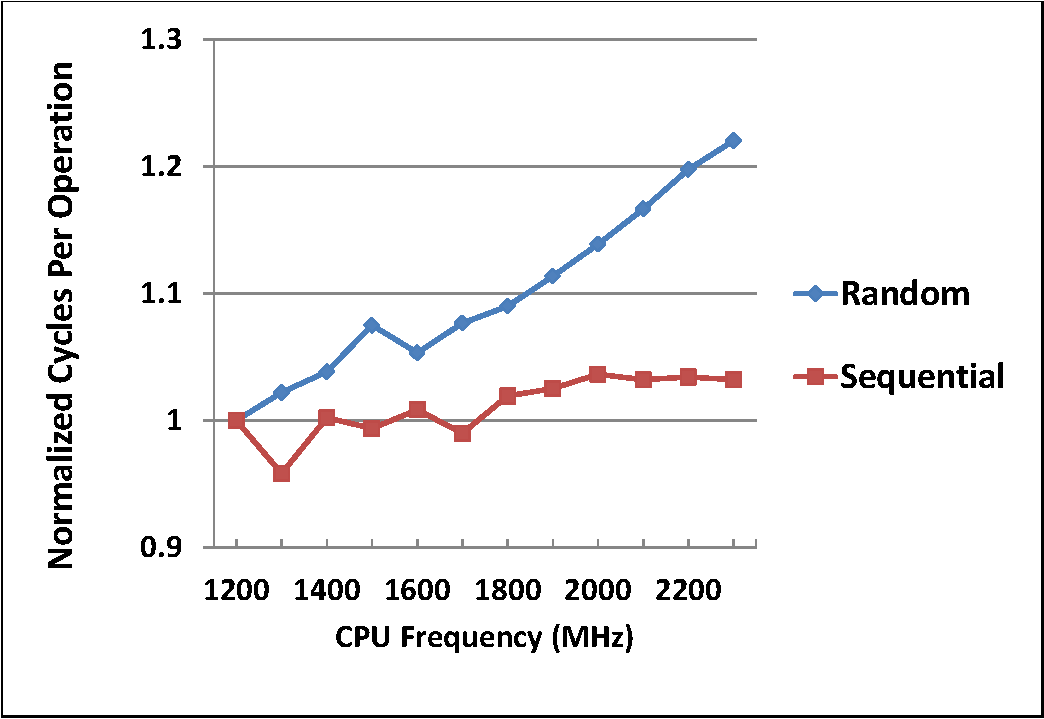
\includegraphics[width=\linewidth]{figs/case-crop.pdf}
  \end{center}
  \vspace{-0.1in}
  \caption{Frequency scaling effect for cache misses}
	\label{fig:case}
\end{figure}

\begin{figure*}[h]
  \begin{center}
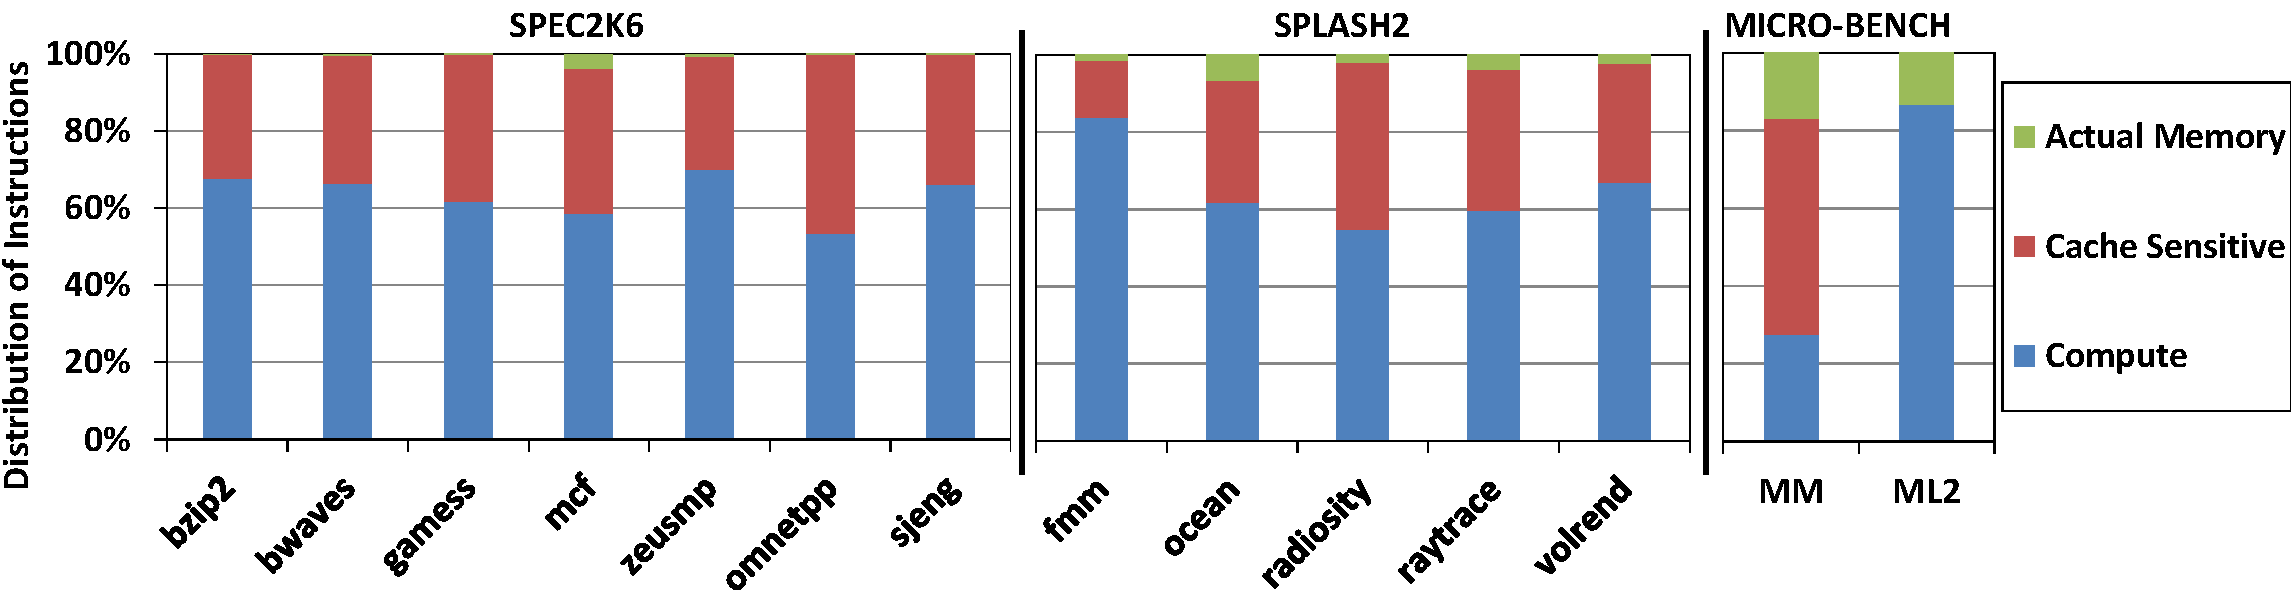
\includegraphics[width=\linewidth]{figs/app-cat-crop.pdf}
  \end{center}
  \vspace{-0.1in}
  \caption{Distribution of Instructions in Applications}
  \label{fig:app-cat}
\end{figure*}



Since both processes do the same amount of computation, the only factor that can affect the performance and efficiency is the memory access pattern. 
If the performance scaled perfectly with CPU frequency, we would expect a nearly flat line, with all cache hits
as we see in the case of sequential access workload in the figure. 
But with random accesses, we see instead that the cycles per operation increase as the frequency increases, 
clearly demonstrating a decrease in the efficiency. This is because of time spent in handling cache misses, and 
CPU is not doing any useful work to hide this latency.
It can be seen that at 2300Mhz, we are ~20\% less efficient than at 1200MHz.
There are two mitigating factors with respect to this issue. First is programming practices -- since cache misses are a well known performance issue, 
many applications are already written to avoid them as much as reasonable. Second is the hardware -- in particular modern processors have both hyperthreading and out of order execution, 
both of these features allowing the processor to potentially work on other instructions while the cache misses
are being served. 

Operating systems however, in this scenario does not take efficient decisions, to actually save energy 
by overriding the default policies. Instead, it still relies on its power
governors to run at higher CPU frequency and thus waste energy. This could be a simple
example, but nonetheless, as we will demonstrate in further sections  with some real workloads, 
the inevitable constraint is memory bandwidth and/or latency, and in these cases a decrease in CPU frequency may very well lead to efficiency gains.




\section{Project phases}\label{sec:plan}
The project will be distributed into multiple phases, but some phases are 
orthogonal so that it can be implemented in parallel among the project members.

\begin{itemize}
\item \textbf{Phase 0:} Picking an application suite representative of typical Linux system (Single/Multi-threaded, I/O, Memory bound).  
\item \textbf{Phase 1:} Profiling the applications and categorizing them into different buckets -- CPU intensive, Memory intensive, I/O intensive. Determine the energy needs for each bucket.
\item \textbf{Phase 2:} Implement framework to collect dynamic information about battery resource, CPU utilization, memory frequency (ACPI and Smart battery interfaces are good place to start). This has to be fed to power governors at specific time intervals to make certain decisions to actually reduce the CPU frequency or go into a lower system power mode. A decision table data structure to be formulated here based on application requirement and actual energy resource available. 
\item \textbf{Phase 2:} Implementing a Linux power governor to support policies/mechanisms for the energy decisions to be taken based on information obtained in Phase 1 and Phase 2. User-space power governors could be a good place to start.  
\item \textbf{Phase 4:} Analyze and compare/reason-out the effects of the energy policies implemented in E-MOS with standard Linux platform. 
\end{itemize}
 
\section{Power Governors Analysis}\label{sec:appl}

\begin{figure*}[h]
  \begin{center}
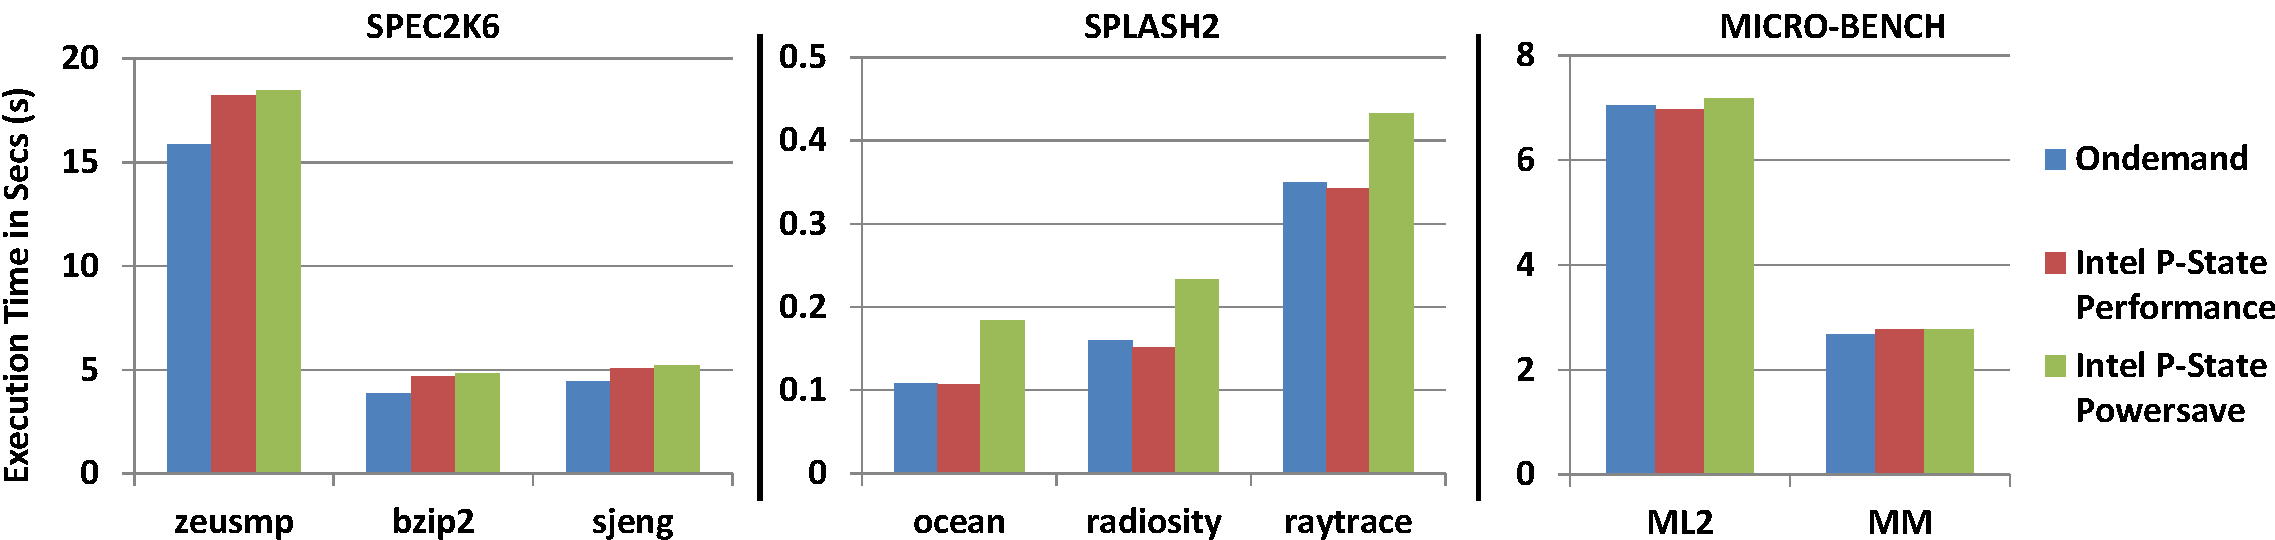
\includegraphics[width=\linewidth]{figs/def-exec-time-crop.pdf}
  \end{center}
  \vspace{-0.1in}
  \caption{Execution time for Linux ondemand and Intel P-state power governors}
  \label{fig:def-perf}
\end{figure*}

The case study in the previous section showed a contrived example and how cache misses are effected 
due to the imperfect frequency scaling in Linux power governors.
In this section, we consider real applications and try to analyze how existing Linux power
governors perform for different class of applications.

\subsection{Application categorization}
We chose applications from  SPEC2006~\cite{spec2006} and SPLASH2~\cite{splash2} to account for both single-threaded and 
multi-threaded applications' analysis. 
We also have written two micro-benchmarks which we call as MICRO-BENCH
suite from now, to exercise 
memory behavior. ML2 is a linked-list traversal workload and 
MM is a workload which has byte accesses larger than
cache line size. 
To first analyze the distribution of instruction in these applications,
we used the PIN~\cite{pin} binary instrumentation tool for profiling.
The PIN tool was modeled to account for total instructions in the application, 
instructions which get hit in the cache and instructions which miss in the cache
and actually access the memory. 
The application profiling was mainly done to figure out
which frequency must be scaled  
based on the time spent by these applications
in CPU or DRAM or Caches.
We could not get Disk (I/O) related instructions and I/O behavior
of applications, as PIN cannot model file system accesses, and
we have no control over the speed at which DISK accesses happen. So, our focus is
mainly on the following three categories:

\begin{itemize} 
\item \textit{Compute Intensive}: The applications which spend most of their execution
time in CPU core and have more computation instructions
between load/stores to the memory. For these applications, CPU
frequency is the important parameter.
\item \textit{Cache Sensitive}: The applications which have more memory access instructions,
but due to the locality of the data accesses, most of them get the data in CPU caches.
For these applications, again CPU frequency is important. 
For our analysis, we assume that, 
CPU cycles will be wasted in getting the data from the caches, whenever
it encounters load or store instructions. 
It is possible that just
by profiling the memory related instructions and not analyzing the cache accesses,
one could misinterpret the application as memory intensive always
and scale the DRAM frequency which we explain below. 
\item \textit{Memory Bound} These are the applications, which have lot of last level cache misses
and the accesses reach memory (DRAM). Increasing the CPU frequency for these applications could 
lead to wastage of energy and for better performance DRAM frequency might have to
be scaled rather than CPU frequency. 
\end{itemize}

Figure~\ref{fig:app-cat} shows the application categorization and distribution of instructions 
across seven SPEC2006 benchmarks, five SPLASH2 benchmarks and two micro-benchmarks. 
We see that SPEC2006 has more compute intensive instructions with some of them
having good cache locality. SPLASH2 has more cache sensitive instructions 
in average with some having good percentage of compute as well as memory related instructions. 
The micro-benchmark MM has lot of cache related instructions and many accessing memory.
ML2 has zero cache access and all of the load/store  instructions access the memory.

\subsection{Power governors performance}

We executed these applications on a Linux kernel with Ondemand~\cite{ondemand2006} power governor
as the default and also ran the applications on two power governors (performance and powersave) 
of Intel's recent P-state~\cite{pstate, rotem2012power} driver \footnote{
Section~\ref{sec:meth} explains the methodology used for performance and energy estimation}. 
We considered Intel's P-state driver, as it has access to turbo boost frequency 
through direct driver interface. Figure~\ref{fig:def-perf} shows the execution time 
of selected benchmarks across all three applications suites (SPEC2K6, SPLASH2 and MICRO-BENCH) for
three discussed power governors. It is seen that, each of the three power governors 
have similar performance even though each has a distinct objective.
Intel P-state performance governor is supposed to boost the performance
with access to turbo boost frequency. Even though, P-state powersave governor 
has slightly worst performance compared to other two, as it tries
to save power by reducing the frequency, the difference is not significant.
The next subsection details on energy efficiency of each of these governors. 

\subsection{Power governors energy efficiency}
\begin{figure}[h]
  \begin{center}
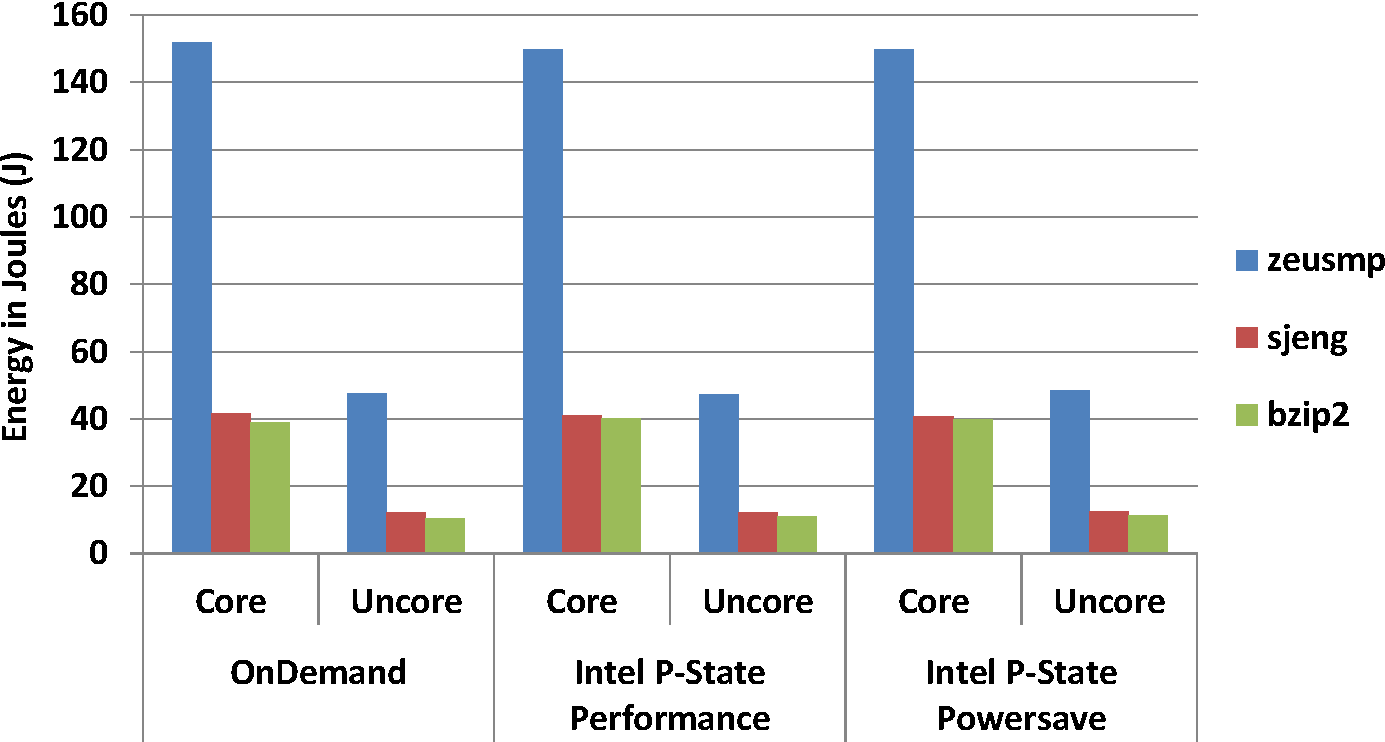
\includegraphics[width=\linewidth]{figs/def-drivers-spec-crop.pdf}
  \end{center}
  \vspace{-0.1in}
  \caption{Energy Consumption for SPEC2006 workloads with ondemand and p-state governors}
  \label{fig:spec-energy}
\end{figure}

As seen with the execution time, we also wanted to analyze
if the power governors perform similar with respect to energy efficiency.
Figure~\ref{fig:spec-energy} shows the energy consumption in Joules for three of the SPEC 2006
benchmarks. We see that the core and encore energy for all the three 
benchmarks across all three governors are similar.  
Figure~\ref{fig:micro-energy} shows similar trend for memory intensive micro-benchmarks.


\begin{figure}[h]
  \begin{center}
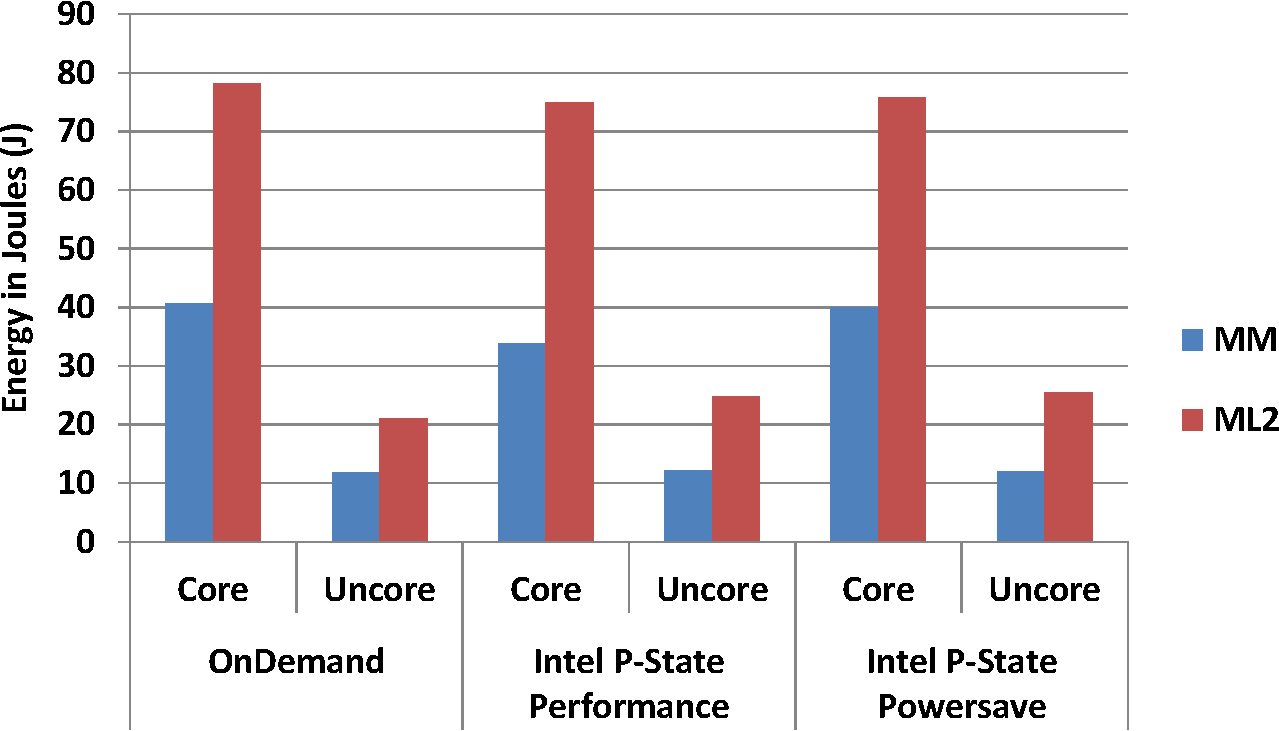
\includegraphics[width=\linewidth]{figs/def-drivers-micro-crop.pdf}
  \end{center}
  \vspace{-0.1in}
  \caption{Energy Consumption for MICRO-BENCH with ondemand and p-state governors}
	\label{fig:micro-energy}
\end{figure}

Figure~\ref{fig:splash-energy} shows energy consumption for SPLASH2 benchmarks.
In case of SPLASH2 benchmarks, it can be seen that for all three workloads, P-state powersave saves more
energy around 2-3 joules compared to other two governors. This complements
why powersave governor had worst execution time than other two. However, still 
the powersave governor does not save significant energy savings even though it reduces 
the CPU frequency to save lot of power.

\begin{figure}[h]
  \begin{center}
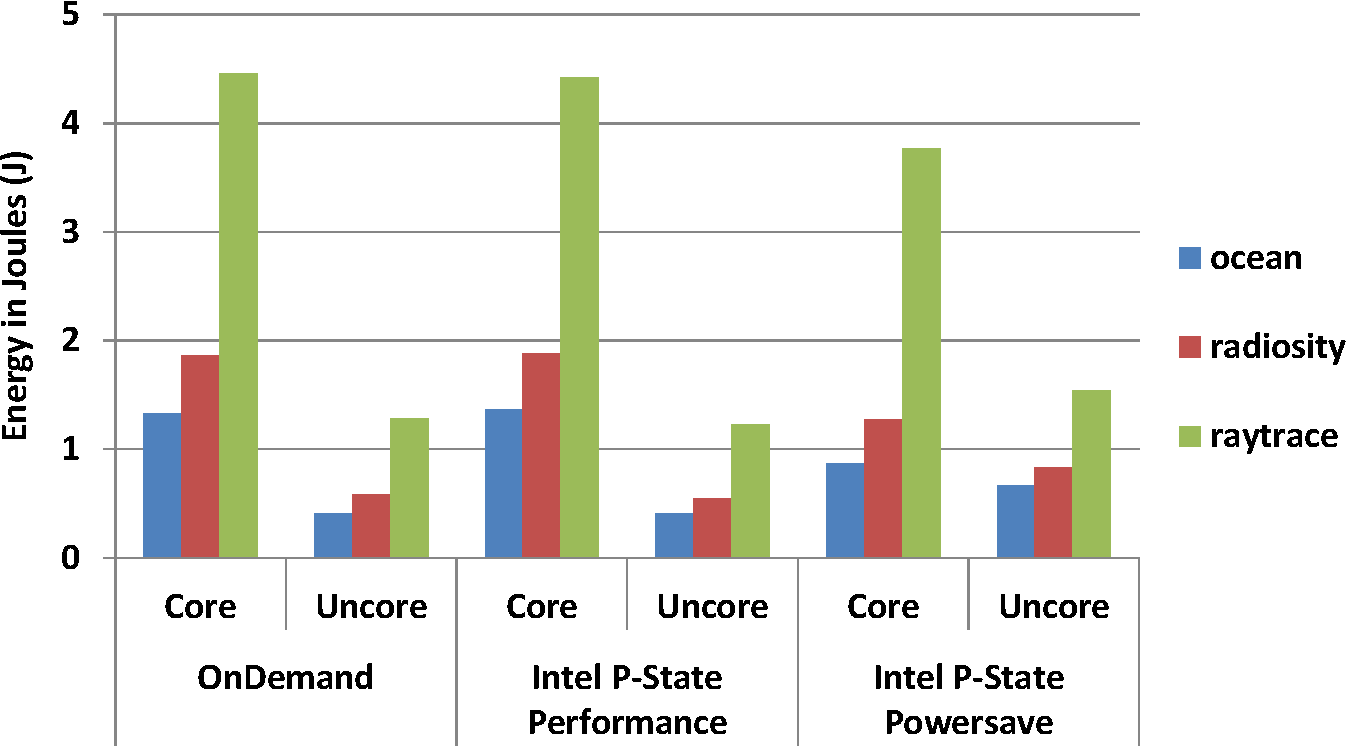
\includegraphics[width=\linewidth]{figs/def-drivers-splash-crop.pdf}
  \end{center}
  \vspace{-0.1in}
  \caption{Energy Consumption for SPLASH2 workloads with ondemand and p-state governors}
  \label{fig:splash-energy}
\end{figure}

\vspace{-0.1in}
The takeaway from this analysis is that: 1) existing Linux power governors 
are optimized only for compute intensive benchmarks;
2) All the three power governors mainly use "race to halt" approach to execute workloads 
fast (scale CPU frequency) and thus save energy;
3) The existing power governors are not application-aware and do not rely
on application characteristics to scale CPU or DRAM frequency;
4) ondemand governor scales frequency on overall system load
rather than individual application requirements;
Based on these takeaways, we believe that Operating systems
should give more freedom to user-space for energy management
and making better policy decisions. User-space has more 
information about applications it is running than
the underlying drivers or hardware.
We now present our model E-MOS, which is an application-aware
energy management model and discuss its implications on OS energy management polices.

\section{Analytical Modeling}\label{sec:analytic}

\fixme{To be added: Decision Table and the graph depicting the model's ideal energy and performance benefits}

Huge essay -- analytic
Huge essay -- analytic
Huge essay -- analytic
Huge essay -- analytic
Huge essay -- analytic
Huge essay -- analytic
Huge essay -- analytic
Huge essay -- analytic
Huge essay -- analytic
Huge essay -- analytic
Huge essay -- analytic
Huge essay -- analytic
Huge essay -- analytic
Huge essay -- analytic
Huge essay -- analytic
Huge essay -- analytic
Huge essay -- analytic
Huge essay -- analytic
Huge essay -- analytic
Huge essay -- analytic
Huge essay -- analytic
Huge essay -- analytic
Huge essay -- analytic
Huge essay -- analytic
Huge essay -- analytic

\begin{table}[h]
\footnotesize
\def\arraystretch{0.52}
\setlength{\tabcolsep}{.30em}
\center
\begin{tabular}{cccc} \toprule
Application & Objective & CPU Freq. & DRAM Freq.  \\ \midrule
Compute Intensive & Energy & Maintain & Decrease \\
Compute Intensive & Performance & Increase & Maintain \\
Cache Sensitive & Energy &  Decrease & Decrease \\ 
Cache Sensitive & Performance &  Maintain & Increase \\ 
Memory Intensive & Energy & Decrease & Maintain \\
Memory Intensive & Performance & Maintain & Increase \\ \midrule

\end{tabular}
\caption{E-MOS Policy Decision Table}\label{tbl:emos-dec}
\end{table}


\begin{figure}[h]
  \begin{center}
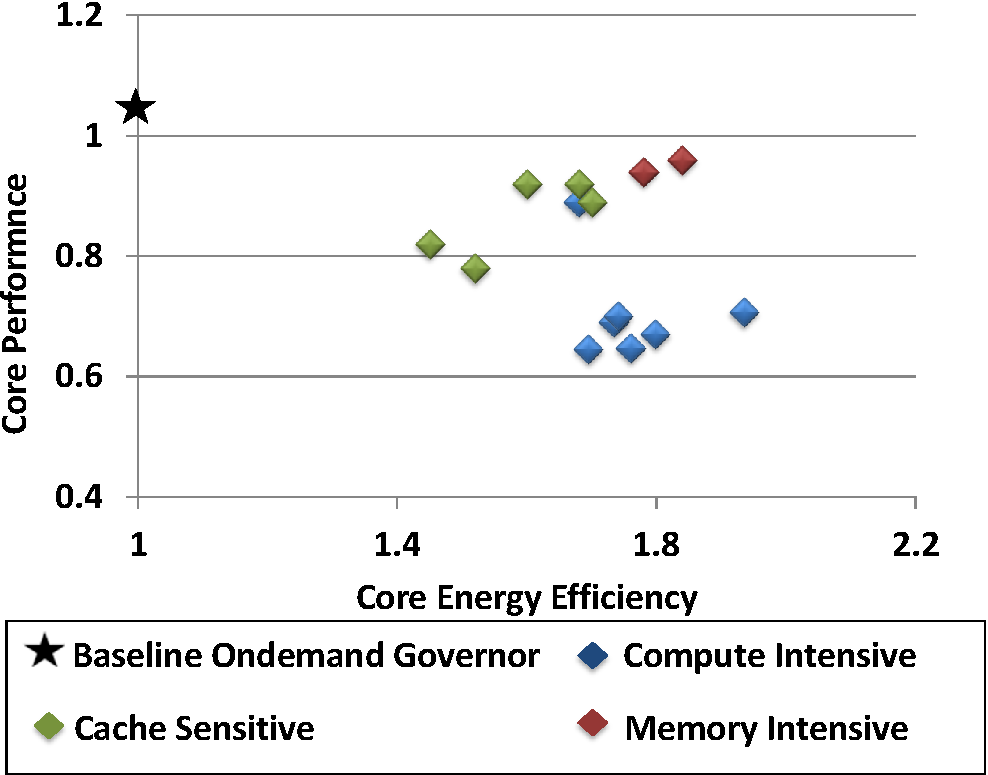
\includegraphics[width=\linewidth]{figs/ana-reduce-crop.pdf}
  \end{center}
  \vspace{-0.1in}
  \caption{Freq reduced by 30\%}
	\label{fig:reduce-freq}
\end{figure}


\begin{figure}[h]
  \begin{center}
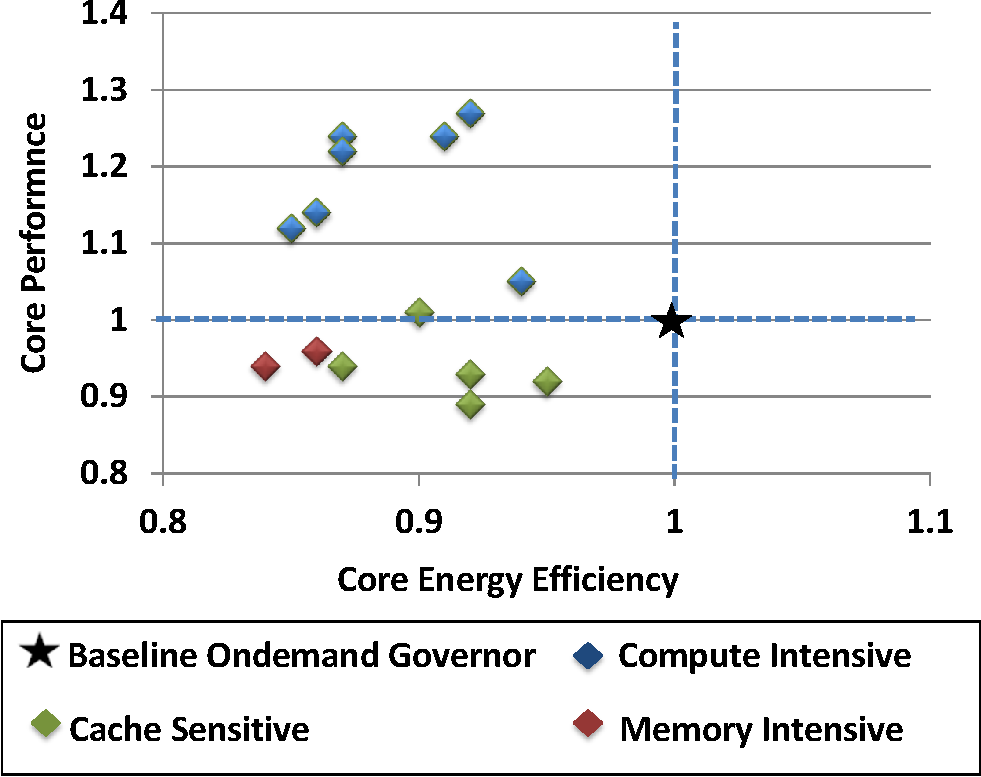
\includegraphics[width=\linewidth]{figs/ana-increase-crop.pdf}
  \end{center}
  \vspace{-0.1in}
  \caption{Freq increased by 30\%}
	\label{fig:increase-freq}
\end{figure}





\section{Methodology and Evaluation}\label{sec:meth}
	This also lists the resources we will be using for our project.

For our study, we will be modifying a stable version of Linux kernel with ACPI and Smart battery interface support. PinTool~\cite{pin} will be used for profiling applications and categorize them into different buckets. To get initial estimates of power/energy consumption of applications, we plan to use two methods -- Our first method uses the ACPI interface to measure the runtime energy (battery) consumption at specific time intervals (epochs) based on the average execution time of all the applications and second method is to use a simulator integrated with energy measurement tool (Just to see whether our measurements co-relate). 
We plan to develop a energy decision table, with category of application on one dimension and concerned energy rule/target on the other. This decision table will be used to develop policies in Linux power governor.  
Evaluation will be done by determining the performance and energy for all the applications with E-MOS implemented. Performance counters (RAPL tool) and again standard ACPI interface for energy measurements will be used.
Finally, we will compare it with runs on standard Linux platform. 



 
\section{Results}\label{sec:results}

Include the User space governor results explaning the decision table 

\section{Related Work}\label{sec:rel}

The Energy Management (EM) area in operating systems constitutes a diverse set of solutions to the problem of ensuring performance while decreasing power usage. 
The Linux kernel has some predefined governors for managing power but many papers have recognized that these general purpose solutions are certainly not optimal, 
and perhaps in some case not even adequate. 
There have been a number of attempts to remedy this and we enlist some of these solutions in this section. Dynamic Voltage Frequency Scaling~\cite{dvfs} has been a 
popular hardware mechanism to save power and boost performance. Zeng et. al~\cite{ecos} focuses on directly managing power usage as one might manage other scarce resources. 
Choi et. al~\cite{decomp} dynamically profile applications to determine a good energy management policy at hardware level. 

\paragraph{Non-Optimal General Purpose EM Policies} It has been recognized that the generic policies for energy management 
implemented in Linux by using the ACPI interface are not always the best performing, or most efficient. For example in the 
context of mobile devices~\cite{and-dvfs}, the on-demand power governor used by the Android operating system does not guarantee 
low power consumption for all workloads. Recently (as of linux 3.9), Intel introduced a P-state driver that is more platform specific 
to overcome some of the issues of the ACPI governors. On the opposite end of the spectrum, we see work done by Yanpei. et. al~\cite{sleepscale} that 
attempts to tackle this issue for datacenter workloads and emphasizes QOS guarantees rather than energy efficiency. Our work focuses on 
providing more dynamic energy management decisions based on the application information. Our work is similar to the work 
in ~\cite{and-dvfs}, in the sense that we use the UserSpace power governor to drive our power policy and compare our implementation with 
the other Linux governors. 

\paragraph{Existing Energy Efficiency Policies} In the case of~\cite{ecos}, energy is treated as another scarce resource and a currency based algorithm is used. 
Processes in this system are allocated a specific amount of power usage, and are given access to various power consuming operations in relation to the amount 
of power they are allocated. However, this is focused largely on the question of optimization of allocation, and not on the question of how to ensure that the energy is productively used.
Other implementations~\cite{and-dvfs, decomp} attempt to form a correlation between the number of memory accesses and ideal operating frequency. They base this 
argument on the fact that some workloads see lower power when executed at higher frequencies. Their experiments show that this is a consequence of the 
number of memory accesses, whose frequency of operation remains constant. By getting a measure of the memory accesses in a workload, 
they use the memory access - CPU frequency correlation to set the operating frequency.
We have a similar approach where we classify workloads depending on how CPU/memory bound and cache sensitive. 
We use this information to make power management decisions for these classified workloads. 

\paragraph{Application Profiling and decomposition} Dynamic voltage and frequency scaling based on application profiling and 
decomposition has been done in Choi. et. al~\cite{decomp}. This idea on profiling is similar to our project’s initial profiling step, but the workload 
is decomposed into two-parts here: On-chip and Off-chip, effectively indicating CPU sensitive and memory sensitive applications respectively. 
It exploits on the idea that different workloads have different power management needs and this statistics could be exploited by the performance 
monitoring unit (PMU) at run-time. They do not implement this in operating system and  overall energy management policy has to still go through kernel 
and the kernel may decide to override the policy based on its decisions. Similarly, Choi et. al~\cite{choi2005fine} work does DVFS for energy conservation 
classifying all the applications based on On-chip and Off-Chip computation ratio. Again this would result in a generic decision, based on ratios calculated offline. 
Power conscious fixed scheduling policy of applications with DVFS based on profiling information has been implemented in Shin et. al~\cite{shin1999power}, 
which again does not integrate the decision making capability to operating systems. Our project aims at embedding this application information 
into energy management decision making policy of operating system kernel and does this based on application needs. 

\section{Conclusion}\label{sec:conc}
Through this project, we aimed to prove that energy efficient power decisions can be made by taking application 
characteristics into account. While our implementation is limited to a static analysis of workloads, our results show that 
this idea does have merit. This concept can be extended to a dynamic implementation by using performance counters and 
libraries like PAPI and interfaces like RAPL continue to make this more accessible. 
\paragraph{}We implemented an analytical model, E-MOS, that can be fed application characteristics and system power requirements 
and would suggest an optimum CPU frequency. E-MOS was designed to balance performance and energy consumption and our 
results show that we can achieve up to 2x energy efficiency with a performance loss of 13\%. Considering that our data 
does not include Intel's turbo frequency boost, there is some room for performance improvements as well.
Overall, a userspace power governor implementation that takes these application features into account has the potential to 
be more energy efficient than current defaults like the ondemand governor, even if it means a small loss in performance.

%\input{architecture}
%\input{compiler}
%\input{related}
%\input{methodology}

\bstctlcite{bstctl:etal, bstctl:nodash, bstctl:simpurl}
\bibliographystyle{IEEEtranS}
\bibliography{main}

\end{document}
